\documentclass[a4paper]{article}

\usepackage[english,czech]{babel} %https://github.com/michal-h21/biblatex-iso690
\usepackage[
   backend=biber      % if we want unicode 
  ,style=iso-authoryear % or iso-numeric for numeric citation method          
  ,babel=other        % to support multiple languages in bibliography
  ,sortlocale=cs_CZ   % locale of main language, it is for sorting
  ,bibencoding=UTF8   % this is necessary only if bibliography file is in different encoding than main document
]{biblatex}
\usepackage[utf8]{inputenc}
\usepackage{fancyhdr}
\usepackage{amsmath}
\usepackage{amssymb}
\usepackage[left=2cm,right=2cm,top=2.5cm,bottom=2.5cm]{geometry}
\usepackage{graphicx}
\usepackage{pdfpages}
\usepackage{url}
\usepackage{float}


\graphicspath{{./datos/graphicos}}
\renewcommand{\refname}{Seznam použité literatury}


\newfloat{customgraph}{Hn}{grp}
\floatname{customgraph}{Graf}

\floatstyle{plaintop}
\newfloat{customtables}{Hn}{tbl}
\floatname{customtables}{Tabulka}

\pagestyle{fancy}
\lhead{Praktikum I - (X) Rychlost šíření zvuku}
\rhead{Vladislav Wohlrath}
\author{Vladislav Wohlrath}

\bibliography{source}

\begin{document}

%\begin{titlepage}
%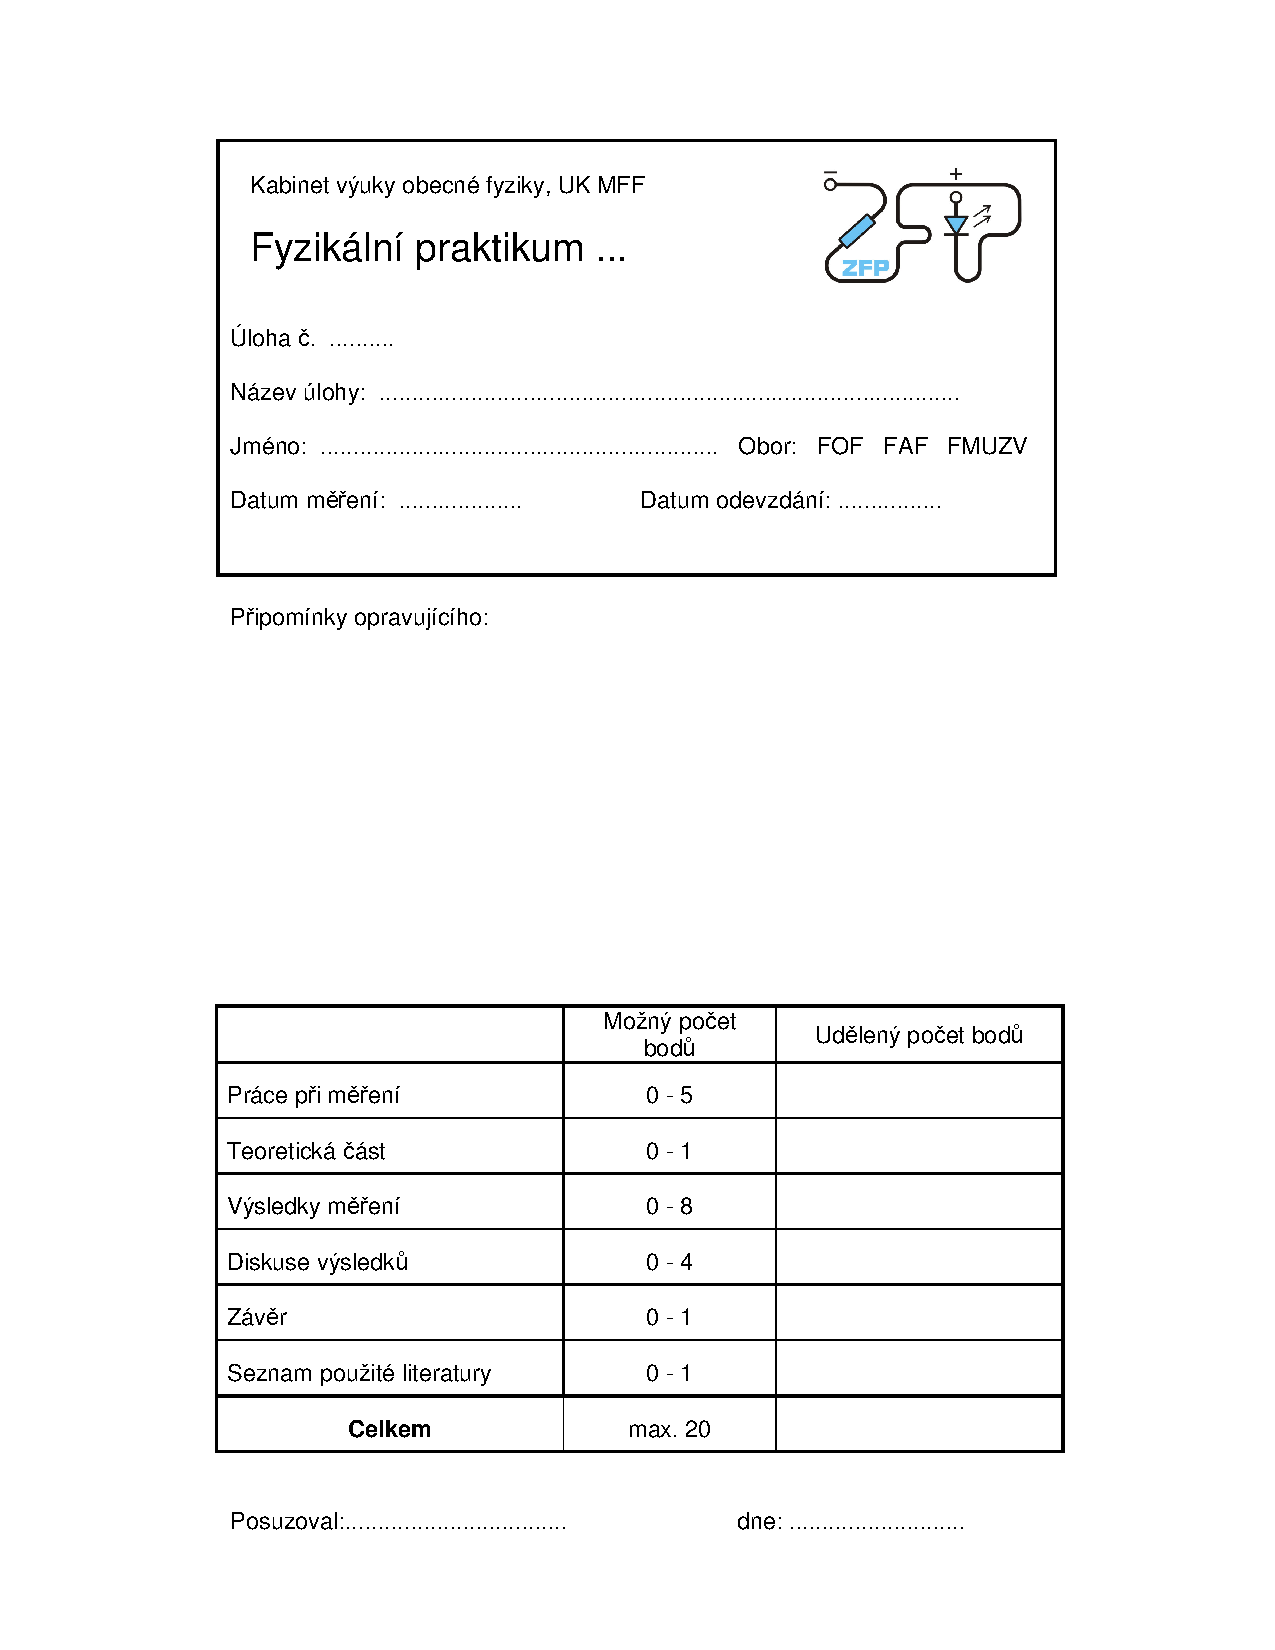
\includepdf[pages={1}]{./graficos/titlelist.pdf}
%\end{titlepage}

\section*{Pracovní úkoly}
\begin{enumerate}
\item Určete rychlost šíření podélných zvukových vln v mosazné tyči metodou Kundtovy trubice. Z naměřené rychlost zvuku stanovte modul pružnosti v tahu E materiálu tyče.
\item Změřte rychlost zvuku ve vzduchu a v oxidu uhličitém pomocí uzavřeného resonátoru. Výsledky měření zpracujte metodou lineární regrese a graficky znázorněte.
\item Vypočítejte Poissonovu konstantu $\kappa$ oxidu uhličitého z naměřené rychlosti zvuku.
\end{enumerate}

%Teoretická část
\section*{Teoretická část}
\subsection*{Kundtova trubice}
Budeme měřit rychlost zvuku v kovové tyči pomocí Kundtovy trubice.
Kundtova trubice je z jedné strany uzavřená skleněná trubice, z druhé strany do ní vložíme tyč ze zkoumaného materiálu, kterou na konci opatříme korkovým pístem.
Do trubice rovnoměrně rozprostřeme korkový prášek a tyč podélně rozkmitáme.
Pokud v trubici vzniklo stojaté vlnění, prášek vytvoří obrazec naznačený v obrázku \ref{obr::obrazectrubice}.
Pokud stojaté vlnění nevzniklo, změníme vzdálenost mezi koncem trubice a korkovým pístem a opakujeme, dokud nevznikne.
Vzdálenost mezi dvěma nejbližšími místy, kde písek nebyl rozmetán, je rovna polovině vlnové délky zvuku.

%\figure \label{obr::obrazectrubice}

Kovovou tyč o délce $l_T$ upevníme v jejím prostředku, pak bude vydávat zvuk o vlnové délce $\lambda_1$ rovné dvojnásobku svojí délky, platí tedy
\begin{equation}
\lambda_1=2 \cdot l_T  \,.
\end{equation}

Při přechodu z jednoho prostředí do druhého si zvuk zachovává svojí frekvenci
\begin{equation}
f_1= \frac{c_1}{\lambda_1}=\frac{c_2}{\lambda_2}=f_2 \,.
\end{equation}
kde $f$ je frekvence, $c$ je rychlost zvuku a dolní indexy 1 a 2 označují prostředí (tyč, vzduch resp.).
Ze známé rychlosti zvuku ve vzduchu a změřených $\lambda_1$, $\lambda_2$ můžeme snadno určit rychlost šíření ve zkoumané tyči.

Pro tenkou tyč platí \cite{ZFP}
\begin{equation}
c_1 = \sqrt{ \frac{E}{\rho}  } \,,
\end{equation}
kde $E$ je modul pružnosti v tahu a $\rho$ je hustota tyče.
Při známé rychlosti zvuku v tyči a její hustoty můžeme vypočítat modul pružnosti 
\begin{equation}
E=c_1^2 \cdot \rho \,.
\end{equation}


\subsection*{Uzavřený rezonátor}
Uzavřený rezonátor je uzavřená dutá kovová trubice s nastavitelnou délkou.
Na jednom jejím konci je připevněn reproduktor napojený na elektronický tónový generátor, na druhém konci je mikrofon napojený na mikroampérmetr.
Rezonance nastává vždy, když je délka rezonátoru celočíselný násobek poloviny vlnové délky zvuku:
\begin{equation} \label{eq::l_na_k}
l=k \cdot \frac{\lambda}{2} \,,  \qquad  k=1, 2, 3, \ldots
\end{equation}
po úpravě
\begin{equation} \label{eq::f_na_k}
f=\frac{c}{2l} \cdot k \,.
\end{equation}

Pokud rezonance nastane, zaznamenáme na mikroampérmetru jako lokální maximum.
Rezonátor je opatřen uzavíratelnými přívody, kterými do něj můžeme napustit měřený plyn.

Rychlost zvuku v plynu budeme měřit dvěma způsoby:
\begin{itemize}
\item S konstantní délkou oscilátoru budeme měnit frekvenci zdroje. Naměřenou závislost \eqref{eq::f_na_k} nafitujeme přímkou $f(k) = a \cdot k$. Z konstanty $a$ určíme rychlost zvuku jako
\begin{equation}
c = 2 \cdot a \cdot k
\end{equation}
\item Při konstantní frekvenci zdroje budeme měnit délku rezonátoru. Po úpravě \eqref{eq::f_na_k} máme
\begin{equation} \label{eq::zavislost_l}
l= \frac{c}{2f} \cdot k  \,.
\end{equation}
Tuto naměřenou závislost nafitujeme přímkou $l(k)= b \cdot k$. Porovnáním s \eqref{eq::zavislost_l} dostaneme
\begin{equation}
c = 2 \cdot f \cdot b \,.
\end{equation}
\end{itemize}

Rychlost zvuku ve vzduchu budeme měřit oběma způsoby.
Rychlost v oxidu uhličitém budeme měřit pouze při konstantní délce rezonátoru.

%Podmínky a měřící přístroje
\section*{Podmínky a použité přístroje}
Teplota v místnosti byla \SI{26.1(4)}{\degreeCelsius}.

Atmosférický tlak byl \SI{983(2)}{\kPa}.

Relativní vlhkost vzduchu byla \SI{36}{\percent}.

Zkoumaná tyč byla vyrobena z mosazi. 
Její délku jsme měřili svinovacím metrem s nejmenším dílkem \SI{1}{\mm}, který považujeme za standardní odchylku měření.

Tabelovaná hodnota hustoty mosazi je podle \cite{converter} v rozmezí \num{8400}--\SI{8750}{\kg\per\m\cubed} v závislosti na jejím složení.
O složení mosazi, z které byla vyrobena  tyč, nemáme žádné informace a proto předpokládáme rovnoměrné rozložení v tomto intervalu (standardní odchylka je rovna délce intervalu dělené odmocninou z dvanácti).
Jako hustotu tyče tedy používáme $\rho =  \SI{8580(100)}{\kg\per\m\cubed}$.

Kundtova trubice měla délku přibližně \SI{74}{\cm}.

Standardní odchylku určení rezonanční frekvence odhadujeme vždy na \SI{3}{\Hz}.

Délku rezonátoru jsme měřili vestavěným pravítkem, standardní odchylku odhadujeme $\sigma_l = \SI{0.5}{\mm}$.

%Výsledky měření
\section*{Výsledky měření}
\subsection*{Kundtova trubice}
Rychlost zvuku ve vzduchu budeme používat hodnotu změřenou metodou uzavřeného rezonátoru při konstantní délce rezonátoru: $c_2 = \SI{00000}{\m\per\s}$~(viz níže).








\subsection*{Uzavřený rezonátor}
Při konstantní délce rezonátoru jsme našli základní frekvenci pro vzduch \SI{213}{\Hz} a pro oxid uhličitý \SI{162}{\Hz}.
Všechny naměřené rezonanční frekvence jsou uvedeny v tabulce \ref{tab::vzduchf} a zaneseny do grafu \ref{grp::graff}.
Frekvence, u nichž není uvedeno číslo $k$, nebyly celočíselnými násobky základní frekvence.
Pravděpodobně se jednalo o tzv. vlčí frekvence, tyto hodnoty jsme vyřadili ze zpracování.


\begin{tabulka}[htbp]
\centering
\begin{tabular}{cc|cc||cc|cc|cc}
\multicolumn{4}{c||}{vzduch} & \multicolumn{6}{c}{oxid uhličitý} \\
$k$ & $f~(\si{\Hz})$ & $k$ & $f~(\si{\Hz})$ & $k$ & $f~(\si{\Hz})$ & $k$ & $f~(\si{\Hz})$ & $k$ & $f~(\si{\Hz})$\\ \hline
1 & 213 & 8 & 1728 & 1 & 162 & 8 & 1347 & 16 & 2692 \\
--- & 324 & 9 & 1941 & 2 & 338 & 9 & 1511 & 17 & 2858 \\
2 & 436 & 10 & 2159 & --- & 486 & 10 & 1681 & 18 & 3028 \\
3 & 650 & 11 & 2375 & --- & 523 & 11 & 1851 & & \\
4 & 872 & 12 & 2597 & 4 & 675 & 12 & 2018 & & \\
5 & 1078 & 13 & 2806 & 5 & 838 & 13 & 2184 & & \\
6 & 1297 & 14 & 3023 & 6 & 1009 & 14 & 2354 & & \\
7 & 1515 & & & 7 & 1179 & 15 & 2524 & & \\
\end{tabular}
\caption{Naměřené rezonanční frekvence při délce rezonátoru $l=\SI{800}{\mm}$}
\label{tab::vzduchf}
\end{tabulka}






\begin{graph}[htbp] 
\centering
% GNUPLOT: LaTeX picture with Postscript
\begingroup
  \makeatletter
  \providecommand\color[2][]{%
    \GenericError{(gnuplot) \space\space\space\@spaces}{%
      Package color not loaded in conjunction with
      terminal option `colourtext'%
    }{See the gnuplot documentation for explanation.%
    }{Either use 'blacktext' in gnuplot or load the package
      color.sty in LaTeX.}%
    \renewcommand\color[2][]{}%
  }%
  \providecommand\includegraphics[2][]{%
    \GenericError{(gnuplot) \space\space\space\@spaces}{%
      Package graphicx or graphics not loaded%
    }{See the gnuplot documentation for explanation.%
    }{The gnuplot epslatex terminal needs graphicx.sty or graphics.sty.}%
    \renewcommand\includegraphics[2][]{}%
  }%
  \providecommand\rotatebox[2]{#2}%
  \@ifundefined{ifGPcolor}{%
    \newif\ifGPcolor
    \GPcolorfalse
  }{}%
  \@ifundefined{ifGPblacktext}{%
    \newif\ifGPblacktext
    \GPblacktexttrue
  }{}%
  % define a \g@addto@macro without @ in the name:
  \let\gplgaddtomacro\g@addto@macro
  % define empty templates for all commands taking text:
  \gdef\gplbacktext{}%
  \gdef\gplfronttext{}%
  \makeatother
  \ifGPblacktext
    % no textcolor at all
    \def\colorrgb#1{}%
    \def\colorgray#1{}%
  \else
    % gray or color?
    \ifGPcolor
      \def\colorrgb#1{\color[rgb]{#1}}%
      \def\colorgray#1{\color[gray]{#1}}%
      \expandafter\def\csname LTw\endcsname{\color{white}}%
      \expandafter\def\csname LTb\endcsname{\color{black}}%
      \expandafter\def\csname LTa\endcsname{\color{black}}%
      \expandafter\def\csname LT0\endcsname{\color[rgb]{1,0,0}}%
      \expandafter\def\csname LT1\endcsname{\color[rgb]{0,1,0}}%
      \expandafter\def\csname LT2\endcsname{\color[rgb]{0,0,1}}%
      \expandafter\def\csname LT3\endcsname{\color[rgb]{1,0,1}}%
      \expandafter\def\csname LT4\endcsname{\color[rgb]{0,1,1}}%
      \expandafter\def\csname LT5\endcsname{\color[rgb]{1,1,0}}%
      \expandafter\def\csname LT6\endcsname{\color[rgb]{0,0,0}}%
      \expandafter\def\csname LT7\endcsname{\color[rgb]{1,0.3,0}}%
      \expandafter\def\csname LT8\endcsname{\color[rgb]{0.5,0.5,0.5}}%
    \else
      % gray
      \def\colorrgb#1{\color{black}}%
      \def\colorgray#1{\color[gray]{#1}}%
      \expandafter\def\csname LTw\endcsname{\color{white}}%
      \expandafter\def\csname LTb\endcsname{\color{black}}%
      \expandafter\def\csname LTa\endcsname{\color{black}}%
      \expandafter\def\csname LT0\endcsname{\color{black}}%
      \expandafter\def\csname LT1\endcsname{\color{black}}%
      \expandafter\def\csname LT2\endcsname{\color{black}}%
      \expandafter\def\csname LT3\endcsname{\color{black}}%
      \expandafter\def\csname LT4\endcsname{\color{black}}%
      \expandafter\def\csname LT5\endcsname{\color{black}}%
      \expandafter\def\csname LT6\endcsname{\color{black}}%
      \expandafter\def\csname LT7\endcsname{\color{black}}%
      \expandafter\def\csname LT8\endcsname{\color{black}}%
    \fi
  \fi
  \setlength{\unitlength}{0.0500bp}%
  \begin{picture}(7936.00,5102.00)%
    \gplgaddtomacro\gplbacktext{%
      \csname LTb\endcsname%
      \put(1078,704){\makebox(0,0)[r]{\strut{} 0}}%
      \csname LTb\endcsname%
      \put(1078,1294){\makebox(0,0)[r]{\strut{} 500}}%
      \csname LTb\endcsname%
      \put(1078,1885){\makebox(0,0)[r]{\strut{} 1000}}%
      \csname LTb\endcsname%
      \put(1078,2475){\makebox(0,0)[r]{\strut{} 1500}}%
      \csname LTb\endcsname%
      \put(1078,3066){\makebox(0,0)[r]{\strut{} 2000}}%
      \csname LTb\endcsname%
      \put(1078,3656){\makebox(0,0)[r]{\strut{} 2500}}%
      \csname LTb\endcsname%
      \put(1078,4247){\makebox(0,0)[r]{\strut{} 3000}}%
      \csname LTb\endcsname%
      \put(1078,4837){\makebox(0,0)[r]{\strut{} 3500}}%
      \csname LTb\endcsname%
      \put(1210,484){\makebox(0,0){\strut{} 0}}%
      \csname LTb\endcsname%
      \put(1526,484){\makebox(0,0){\strut{} 1}}%
      \csname LTb\endcsname%
      \put(1843,484){\makebox(0,0){\strut{} 2}}%
      \csname LTb\endcsname%
      \put(2159,484){\makebox(0,0){\strut{} 3}}%
      \csname LTb\endcsname%
      \put(2476,484){\makebox(0,0){\strut{} 4}}%
      \csname LTb\endcsname%
      \put(2792,484){\makebox(0,0){\strut{} 5}}%
      \csname LTb\endcsname%
      \put(3109,484){\makebox(0,0){\strut{} 6}}%
      \csname LTb\endcsname%
      \put(3425,484){\makebox(0,0){\strut{} 7}}%
      \csname LTb\endcsname%
      \put(3742,484){\makebox(0,0){\strut{} 8}}%
      \csname LTb\endcsname%
      \put(4058,484){\makebox(0,0){\strut{} 9}}%
      \csname LTb\endcsname%
      \put(4375,484){\makebox(0,0){\strut{} 10}}%
      \csname LTb\endcsname%
      \put(4691,484){\makebox(0,0){\strut{} 11}}%
      \csname LTb\endcsname%
      \put(5007,484){\makebox(0,0){\strut{} 12}}%
      \csname LTb\endcsname%
      \put(5324,484){\makebox(0,0){\strut{} 13}}%
      \csname LTb\endcsname%
      \put(5640,484){\makebox(0,0){\strut{} 14}}%
      \csname LTb\endcsname%
      \put(5957,484){\makebox(0,0){\strut{} 15}}%
      \csname LTb\endcsname%
      \put(6273,484){\makebox(0,0){\strut{} 16}}%
      \csname LTb\endcsname%
      \put(6590,484){\makebox(0,0){\strut{} 17}}%
      \csname LTb\endcsname%
      \put(6906,484){\makebox(0,0){\strut{} 18}}%
      \csname LTb\endcsname%
      \put(7223,484){\makebox(0,0){\strut{} 19}}%
      \csname LTb\endcsname%
      \put(7539,484){\makebox(0,0){\strut{} 20}}%
      \put(176,2770){\rotatebox{-270}{\makebox(0,0){\strut{}$f (\si{\Hz})$}}}%
      \put(4374,154){\makebox(0,0){\strut{}$k$}}%
      \csname LT0\endcsname%
      \put(3742,3184){\rotatebox{37}{\makebox(0,0)[l]{\strut{}vzduch}}}%
      \csname LT1\endcsname%
      \put(4849,2534){\rotatebox{28}{\makebox(0,0)[l]{\strut{}oxid uhličitý}}}%
    }%
    \gplgaddtomacro\gplfronttext{%
    }%
    \gplbacktext
    \put(0,0){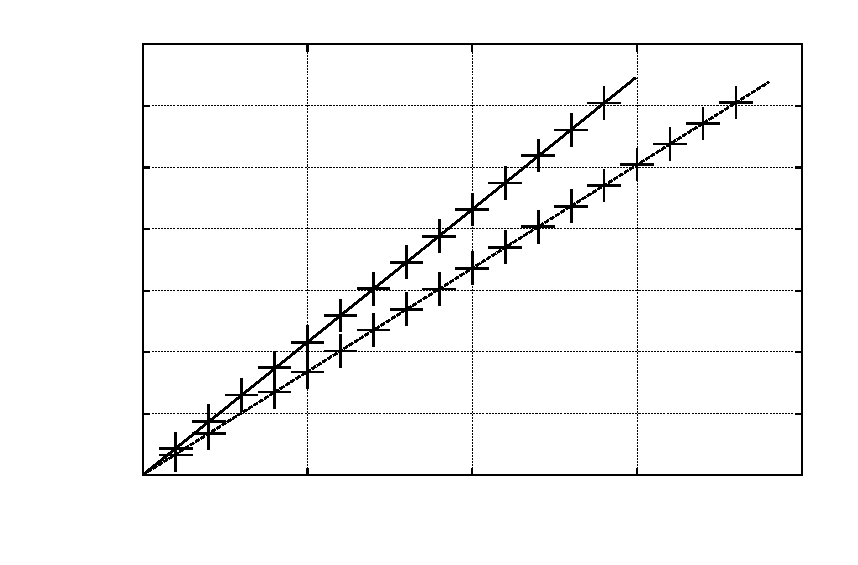
\includegraphics{graffrekvence}}%
    \gplfronttext
  \end{picture}%
\endgroup

\caption{Naměřená závislost rezonanční frekvence $f$ na čísle $k$ (viz rovnice \eqref{eq::f_na_k}) při délce rezonátoru \SI{800}{\mm}}
\label{grp::graff}
\end{graph}

\begin{graph}[htbp] 
\centering
% GNUPLOT: LaTeX picture with Postscript
\begingroup
  \makeatletter
  \providecommand\color[2][]{%
    \GenericError{(gnuplot) \space\space\space\@spaces}{%
      Package color not loaded in conjunction with
      terminal option `colourtext'%
    }{See the gnuplot documentation for explanation.%
    }{Either use 'blacktext' in gnuplot or load the package
      color.sty in LaTeX.}%
    \renewcommand\color[2][]{}%
  }%
  \providecommand\includegraphics[2][]{%
    \GenericError{(gnuplot) \space\space\space\@spaces}{%
      Package graphicx or graphics not loaded%
    }{See the gnuplot documentation for explanation.%
    }{The gnuplot epslatex terminal needs graphicx.sty or graphics.sty.}%
    \renewcommand\includegraphics[2][]{}%
  }%
  \providecommand\rotatebox[2]{#2}%
  \@ifundefined{ifGPcolor}{%
    \newif\ifGPcolor
    \GPcolorfalse
  }{}%
  \@ifundefined{ifGPblacktext}{%
    \newif\ifGPblacktext
    \GPblacktexttrue
  }{}%
  % define a \g@addto@macro without @ in the name:
  \let\gplgaddtomacro\g@addto@macro
  % define empty templates for all commands taking text:
  \gdef\gplbacktext{}%
  \gdef\gplfronttext{}%
  \makeatother
  \ifGPblacktext
    % no textcolor at all
    \def\colorrgb#1{}%
    \def\colorgray#1{}%
  \else
    % gray or color?
    \ifGPcolor
      \def\colorrgb#1{\color[rgb]{#1}}%
      \def\colorgray#1{\color[gray]{#1}}%
      \expandafter\def\csname LTw\endcsname{\color{white}}%
      \expandafter\def\csname LTb\endcsname{\color{black}}%
      \expandafter\def\csname LTa\endcsname{\color{black}}%
      \expandafter\def\csname LT0\endcsname{\color[rgb]{1,0,0}}%
      \expandafter\def\csname LT1\endcsname{\color[rgb]{0,1,0}}%
      \expandafter\def\csname LT2\endcsname{\color[rgb]{0,0,1}}%
      \expandafter\def\csname LT3\endcsname{\color[rgb]{1,0,1}}%
      \expandafter\def\csname LT4\endcsname{\color[rgb]{0,1,1}}%
      \expandafter\def\csname LT5\endcsname{\color[rgb]{1,1,0}}%
      \expandafter\def\csname LT6\endcsname{\color[rgb]{0,0,0}}%
      \expandafter\def\csname LT7\endcsname{\color[rgb]{1,0.3,0}}%
      \expandafter\def\csname LT8\endcsname{\color[rgb]{0.5,0.5,0.5}}%
    \else
      % gray
      \def\colorrgb#1{\color{black}}%
      \def\colorgray#1{\color[gray]{#1}}%
      \expandafter\def\csname LTw\endcsname{\color{white}}%
      \expandafter\def\csname LTb\endcsname{\color{black}}%
      \expandafter\def\csname LTa\endcsname{\color{black}}%
      \expandafter\def\csname LT0\endcsname{\color{black}}%
      \expandafter\def\csname LT1\endcsname{\color{black}}%
      \expandafter\def\csname LT2\endcsname{\color{black}}%
      \expandafter\def\csname LT3\endcsname{\color{black}}%
      \expandafter\def\csname LT4\endcsname{\color{black}}%
      \expandafter\def\csname LT5\endcsname{\color{black}}%
      \expandafter\def\csname LT6\endcsname{\color{black}}%
      \expandafter\def\csname LT7\endcsname{\color{black}}%
      \expandafter\def\csname LT8\endcsname{\color{black}}%
    \fi
  \fi
  \setlength{\unitlength}{0.0500bp}%
  \begin{picture}(5668.00,3968.00)%
    \gplgaddtomacro\gplbacktext{%
      \csname LTb\endcsname%
      \put(946,704){\makebox(0,0)[r]{\strut{} 700}}%
      \csname LTb\endcsname%
      \put(946,1454){\makebox(0,0)[r]{\strut{} 750}}%
      \csname LTb\endcsname%
      \put(946,2204){\makebox(0,0)[r]{\strut{} 800}}%
      \csname LTb\endcsname%
      \put(946,2953){\makebox(0,0)[r]{\strut{} 850}}%
      \csname LTb\endcsname%
      \put(946,3703){\makebox(0,0)[r]{\strut{} 900}}%
      \csname LTb\endcsname%
      \put(1977,484){\makebox(0,0){\strut{} 13}}%
      \csname LTb\endcsname%
      \put(3175,484){\makebox(0,0){\strut{} 14}}%
      \csname LTb\endcsname%
      \put(4373,484){\makebox(0,0){\strut{} 15}}%
      \put(176,2203){\rotatebox{-270}{\makebox(0,0){\strut{}$l(\si{\mm})$}}}%
      \put(3174,154){\makebox(0,0){\strut{}$k$}}%
    }%
    \gplgaddtomacro\gplfronttext{%
    }%
    \gplbacktext
    \put(0,0){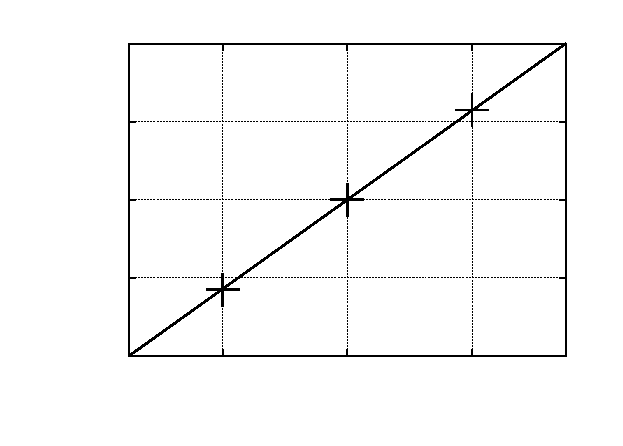
\includegraphics{grafdelka}}%
    \gplfronttext
  \end{picture}%
\endgroup

\caption{Délky rezonátoru, při kterých nastala rezonance (vzduch, $f=\SI{3025}{\Hz})$ }
\label{grp::grafl}
\end{graph}

%Diskuze výsledků
\section*{Diskuze}

%Závěr
\section*{Závěr}

Všechny uvedené odchylky jsou standardní ($P=\num{0.68}$).


\printbibliography[title={Seznam použité literatury}]

\end{document}